% 项目用到的技术与工具简介

\chapter{技术、框架与工具}
  \label{chap:技术与工具}
    本章主要介绍了项目所用到的技术和工具,技术包括:
    \begin{itemize}
      \item HTTP
      \item JSON 与 XML
      % \item Apache 服务器的配置
      % \item Nodejs 与 npm
      % \item MongoDB
      \item 前端技术
      \item H5
      \item CSS3 与 Less
      \item ES5,ES6
      \item 前端库与框架
      \item jQuery
      \item Bootstrap
      \item MVC 与 AngularJS
    \end{itemize}

    工具包括:

    \begin{itemize}
      \item Sublime Text3
      \item Chrome
      \item 微信 Web 开发者工具
      \item Git
    \end{itemize}

    \section{技术与框架}
      \label{sec:技术框架}
        \subsection{HTTP}
          \label{subsec:http}
            \subsubsection{HTTP 简介}
              \label{subsubsec:http_简介}
                HTTP(HyperText Transport Protocol)是超文本传输协议,规定了浏览器和服务器的通信的规则。RFC 系列文档收录了互联网通信的一些规范,其中 RFC2612 记录了 HTTP 协议的规范。

                当我们在浏览器中键入了一个网址的时候,都发生了什么?首先浏览器把网址发送到某个 DNS 服务器,DNS 服务器负责将网址解析成 ip 地址,然后浏览器再向 ip 地址对应的服务器发送请求,服务器接收到请求,返回你想要的资源,通常是网页的形式。其实从服务器那边传过来的,不只有网页,还有一些头信息,这些信息对客户是不可见的,但却十分重要,这些信息反映了用到的 http 协议及其版本、缓存相关的设置、传输的编码等、获取信息的状态及状态码等,这些信息都可以从 Chrome 的调试工具里面看到。

            \subsubsection{开发者如何使用 HTTP}
              \label{subsubsec:开发者如何使用_http}
                理解 HTTP 协议对于网站开发者,无论是前端还是后台都十分重要。
                \par
                对于前端工作者,我们时常需处理与后台的数据传输问题,而与后台的交互离不开 Ajax (Asynchronous JavaScript And XML),我们开发用到的一些框架(如 jQuery)都集成了 Ajax 请求的方法,如果我们理解了 HTTP 协议,就不会对 Ajax 请求所需要的那些参数感到陌生,我们也常常遇到请求失败等的问题,此时我们就需要在浏览器中去查看 Get 请求或 POST 的构建是否正确。
                \par
                对于后台开发者,理解 HTTP 请求就更重要了,因为后台要负责 GET 请求和 POST 请求的接收和处理,需要设置 cookie 、回话管理、资源的缓存、缓存的时间等等。
                \par
                因此,我们如果要想开发网站,就要花时间去理解 HTTP 协议,这样才能让我们走得更远。

        \subsection{JSON 和 XML}
          \label{subsec:json_和_xml}
            \subsubsection{前后分离的开发模式}
              \label{subsubsec:前后分离的开发模式}
                现在的项目开发流行一种新模式,即前后端分离,这种开发方法可以降低耦合,提高开发效率,让不同的程序员更加专注自己擅长的地方,如后端工程师只需专注于数据的增删改查等数据库操作,前端只负责页面样式、动画特效等。前后端的数据采用的数据格式主要有两种:JSON 和 XML,主流都是在用 JSON,少部分仍在使用 XML,例如微信的开发。
            \subsubsection{XML}
              \label{subsubsec:XML}
                XML(Extensible Markup Language) 是表示数据的一种格式,特点是采用了类似 HTML 标签的方式把数据包裹起来,不同的地方在于标签名可以自定义,这有点类似 AngularJS 的自定义命令,XML 可以表示出所有的数据结构:对象和数组,语法严格,但是用 XML 标签构造的数据携带了大量的无用的标签,是 JSON 未出来之前的很流行的一种数据传输格式。尽管 JSON 更简洁,但 XML 还未完全退出,这里之所以提到 XML 是因为微信开发仍在采用,微信的事件推送、消息机制的 POST 数据,都是 XML 格式。
            \subsubsection{JSON}
              \label{subsubsec:JSON}
                JSON(JavaScript Object Notation, JavaScript 对象表示法) 是 JavaScript 语言的对象的表示方法,由 Douglas Crockford 提出的,《JavaScript: The Good Parts》的作者。JSON 数据格式十分简洁,只需 "\{"、"["、","、":" 这四中符号就可以表示出任意的结构。"\{" 大括号用来表示对象的集合,是由一些键值对用逗号隔开组成的;"," 逗号用来分隔键值对;":" 冒号用来分隔键与值;"[" 中括号用来包裹对象,即一些大括号的组合。相比于 XML,用最少的额外信息表示了最多的数据,节省了带宽,数据呈现也更加友好,更加直观,现在在被大量采用。

        \subsection{前端技术}
          \label{subsec:前端技术}
            前端的开发所用到的技术为:HTML, CSS 和 JavaScript, HTML 负责内容(Content), CSS负责表现(Presentation),JavaScript负责行为(Behavior),这三种技术相互配合,形成了浏览器上绚丽的网页。

            \subsubsection{HTML}
              \label{subsubsec:html}
                HTML 是网页采用的标记语言,全称为: HyperText Markup Language, 超文本标记语言,标记语言指的是用一些符号去标记一些文字、图片路径等,写成纯文本格式的文件,然后再用某种解析器把文件渲染成华丽的页面,展现出来,超文本指的是展现的内容不仅仅是文字,还可以是图片、声音、视频等丰富的多媒体内容。

            \subsubsection{CSS}
              \label{subsubsec:css}
                CSS 全称是 Cascade Style Sheet,即层叠样式表,用来控制页面的样式,HTML 写的页面要想华丽地展现必须靠 CSS 去控制样式,控制布局,例如浮动、大小、位置、颜色、字体等。

            \subsubsection{Less}
              \label{subsubsec:less}
                Less 语言是 CSS 的升级版,让写的代码更易维护,用 Less 写 样式非常舒服,它支持嵌套、变量、表达式等,可以提升开发效率。但是,Less 文件不能被浏览器直接解析,需要通过 Less 预编译器编译成 CSS 文件才能在浏览器中执行。

            \subsubsection{JavaScript}
              \label{subsubsec:javascript}
                JavaScript 是一门编程语言,而一种语言的运行必须要有运行环境,运行环境提供了该语言的编译、调试工具以及一些常用的扩展库。JavaScript 的运行环境是浏览器和 Nodejs(服务器端的运行环境)。通常来说,前端的 JavaScript 包括了一下三部分:
                \begin{itemize}
                  \item ECMAScript (核心)
                  \item DOM(Document Object Model, 文档对象模型)
                  \item BOM(Browser Object Model,浏览器对象模型)
                \end{itemize}
                \par
                ECMAScript 是标准的 JavaScript 规范,因为早在 ECMAScript 之前,JavaScript 有很多版本,各个主流浏览器厂商的 JavaScript 语法都不太一样,ECMAScript 是为了规范化 JavaScript 而诞生的,目前最新版是 ES6, 2015 年推出。DOM 是文档对象模型,JavaScript 作为前端的语言,被赋予了更多的功能,DOM 让 JavaScript 有了操作 HTML 文档的能力,获用于获取元素和改变元素。BOM 给 JavaScript 赋予了操作浏览器的功能,例如历史记录、URL解析和跳转、计时器等。

        \subsection{H5}
          \label{subsec:h5}
            H5 是现在很流行的一个词,狭义上说,H5 就是 HTML 的最新版,而从广义上说, H5 也包括了 CSS3,ES5甚至ES6 等前端开发的一系列技术的集合,H5 应用就是用这些新技术开发的应用。
            \par
            H5 为什么这么火?H5 新增了很多特性,让开发更加方便,同时页面的展现更加华丽。H5 主要新增了如下的特性:
            \begin{itemize}
              \item 更多的语义标签
              \item 地理位置
              \item Canvas 绘图
              \item Web 存储
              \item 更多的表单
              \item ...
            \end{itemize}
            \subsubsection{语义标签}
              \label{subsubsec:语义标签}
                H5 提供了诸如 <article>, <section>, <figure>, <video> 等很多语义化的标签,这样可以减少 class 属性的叠加,也让 HTML 代码更易读。

            \subsubsection{地理位置 API}
              \label{subsubsec:地理位置_api}
                利用地理位置 API 可以获取用户的位置信息甚至可以调用地图显示位置,一些移动端的应用就是通过这样的方法实现诸如查找附近的商家等功能。

            \subsubsection{Canvas 绘图}
              \label{subsubsec:canvas_绘图}
                Canvas 绘图也是很强大的功能,主要用 JavaScript 绘制,呈现华丽的效果,一些统计图的 JS 库就是用 canvas 实现的,例如百度的 Echarts。

            \subsubsection{Web 存储}
              \label{subsubsec:web_存储}
                本地存储对于 Web 应用来说非常重要,至少有如下优点:
                \begin{itemize}
                  \item 减少服务器压力
                  \item 节约客户端流量
                  \item 访问速度更快
                \end{itemize}
                \par
                本地存储一直追寻的目标是:容量要足够大,数据的持久化(页面刷新),不会随着每次HTTP请求发送,跨浏览器(各个浏览器通用),不需第三方插件等,后面两个是之前的本地存储方案的问题。H5 新增的本地存储几乎解决了上面的问题,例如 localStorage 的最大容量可以达到 5MB,而且可以持久化存储,使用也十分方便。在 Chrome 的调试工具中,Application 一栏可以查看到本地存储的信息,如图 \ref{fig:cr_application}。除了 localStorage ,还有更强大的数据库存储的方式,例如 WebSQL, IndexedDB更多参见 \ref{subsubsec:web_存储} 一节。

            \subsubsection{更多的表单}
              \label{subsubsec:更多的表单}
                H5新增了可以输入时间、日期、搜索框、数字等的表单,这些表单更加智能,例如,日期输入框:<input type="date">,输入框的右侧有一个下拉框,单击可以弹出日期选择框来选择日期。如图 \ref{fig:h5_date}
                \begin{figure}[H]
                  \centering
                  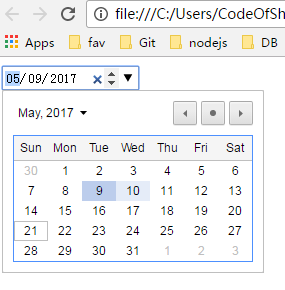
\includegraphics[width=5cm]{./img/h5_date.png}
                  \caption{H5 的日期输入表单}
                  \label{fig:h5_date}
                \end{figure}

                这些输入框还支持占位文本,一些网站的的输入框中一般会有提示字符,这是通过 input 标签的 placeholder属性设置的,如图 \ref{fig:h5_placeholder}
                \begin{figure}[H]
                  \centering
                  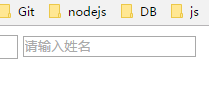
\includegraphics[width=5cm]{./img/h5_placeholder.png}
                  \caption{H 5 的占位文本}
                  \label{fig:h5_placeholder}
                \end{figure}
                当然,H5 还有很多特性,这里不一一列举。

        \subsection{CSS 3}
          \label{subsec:css_3}
            CSS 3 是最新的 CSS 标准,新增了丰富而强大的功能,圆角边框、颜色渐变、弹性盒子、动画等,我的项目中主要采用了圆角边框的特性。圆角边框看起来很美观,实现起来也很简单,常见于一些搜索框,如图 \ref{fig:h5_borderradius}。
            \begin{figure}[H]
              \centering
              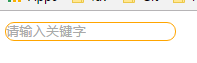
\includegraphics[width=5cm]{./img/h5_borderradius.png}
              \caption{圆角边框特性}
              \label{fig:h5_borderradius}
            \end{figure}

        \subsection{ES 5 和 ES 6}
          \label{subsubsec:es_5_和_es_6}
            \ref{subsubsec:javascript} 一节简要介绍了 JavaScript,我们知道 ECMAScript 是 JavaScript 的标准版本,简称 ES,目前的最新版是 ES6, 2015 年推出,也称 ES2015,但还未大量应用,目前的大部分框架仍是采用上个 ES 版本——ES5。ES 6 相比于 ES5添加了很多特性,比如支持显式地构造类,多了 class 关键词;有了块级作用域与 let 关键字;增加了遍历数组值的语法:of 关键字;增加了强大的 Generator 函数,让异步代码的书写更加容易,也可以用于构造"无限"数列, 这里的无限并不是一次性产生整个数列,而是可以放在循环中,按需要产生。
            \par
            新标准的诞生意味着框架的大规模更新,前端框架如 Angular2 ,基于 Nodejs 的后端框架如 KOA(Express 的下一代)。前端领域发展迅速,我们要顺应时代潮流,不断学习新技术。

        \subsection{前端库与框架,MVC}
          \label{subsec:前端库与框架}
            直接用 HTML,CSS,和 JavaScript 三种技术就可以开发网页。不过,如果要开发大型的应用,会非常难维护,代码量也会很巨大,因此,随着技术的发展,前端领域诞生了大量的库和框架,让开发应用更迅速,也更易维护,且大部分都是开源免费的,可以直接上 Github 上下载源码。那么什么是库,什么是框架呢?
            \par
            库是一些函数的集合,前端领域也包括样式库,如 Bootstrap, 提供了封装好了的一些常用功能,例如方便地设置漂亮的样式、动画,方便地获取与设置元素等,而且在一个项目中一般可以同时使用多个库,只要命名空间不重复即可。
            \par
            框架的使用直接影响到整个项目的架构。一个框架规范了整个项目的布局结构,提供了更高层次的抽象,也有了更多的概念。我们如果只开发一个十分简单的应用,项目结构完全可以由 img 文件夹、css 文件夹, js 文件夹和一些 html 文件构成,这样的设计只是根据文件的类型来划分的,没有所谓的抽象与概念,而如果采用框架来开发,项目结构就要遵循框架的规范,一个项目只能引入一个框架,而且有了众多的概念,例如:模板、控制器等,而且一个框架中可以引入多个库。
            \par
            目前主流的框架通常是基于 MVC 的,M(Module) 指的是模型,V(View) 是视图,C(Controller) 是控制器。模型一般负责数据库操作,控制器负责指挥分配,如:路由配置,为模板填充数据等,而视图就是 html 及其样式文件。这样划分项目的有很多的好处,数据、业务逻辑与模板视图分离,让代码更以维护。以往的动态网页会把代码逻辑与视图全部都写在一起,这样整个页面非常庞大,调试代码不好找,样式也不好控制,而数据与模型分开后,开发人员就可以更加专注,样式出问题了,就只管调样式,样式中没有逻辑,也好定位,同样,逻辑出了问题,只管调逻辑,而不用在意样式。
            \par
            但使用框架同样也有很多弊端,框架有很强的约束性,这要求我们要严格遵守,有时一个字母的大小写弄错都会出问题。出问题了不要紧,如果能很快定位到代码也可以,就怕定位不到代码,而是定位到上万行代码的框架中,这样就造成了调试的极度困难,只能对着文档一点点找错误,找不到还得在网上查阅大量资料,有时查阅大量资料还查不到,因为自己出现的问题很小,别人还没遇到,有时查到资料,但是怎么看也看不懂,因为不理解原理,这时又得花时间去学框架的原理,有时甚至要看源代码,而源代码很多地方又使用了很多高级的 JavaScript 功能,此时又得去花大量时间学习 JavaScript, 你看,就因为一个很小的问题,而花费了如此长的时间去修复,有时还修复不了,而且与其他库共用时也会产生问题。
            \par
            以上的问题在我的项目开发过程中我都遇到过,有时就是简单的几行代码,一旦出错,要花好久才找到,耽误了大量的时间,因此,用好框架是需要积累经验的,积累常见的错误,不可能短时间上手的。不过,这次的项目仍采用了框架 AngularJS, 我更多的关注了框架的优点,学习框架的理念,我相信用熟框架后可以大大提升开发速度。下面来介绍下本次项目用到的库与框架。

        \subsection{Bootstrap}
          \label{subsec:Bootstrap}
            Bootstrap 是一款非常优秀、广泛运用的一款前端库,是由 Twitter 的两位前员工 Mark Otto 和 Jacob Thornton 开发,在 2010 年 8 月面世。Bootstrap 总结了常见的样式与动画,可以快速搭建起网站,样式简洁、大气、美观,如图 \ref{fig:bootstrap}
            \begin{figure}[H]
              \centering
              
\includegraphics[width=10cm]{./img/bootstrap.png}
              \caption{简洁大方的 Bootstrap}
              \label{fig:bootstrap}
            \end{figure}

        \subsection{jQuery}
          \label{subsec:jquery}
            jQuery 是目前最流行的 JavaScript 库,2006 年 1 月 14 日诞生,作者为 John Resig。这是一个轻量的库,但功能强大。jQuery 有很多优秀的特性,几乎是前端开发必备的 JavaScript 库。我喜欢 jQuery 最主要的原因是它代码简洁,强大的 DOM 操作,还支持连缀、隐式遍历等功能。他的可以让我专注于功能,加快开发速度。我的项目的上个版本没有采用框架,全部都是用 jQuery 写的,但由于项目功能复杂,开发到最后实在难以维护,于是又换成了 AngularJS 框架,但有些地方仍在采用 jQuery ,因为 jQuery 的 DOM 操作是其他框架无法比拟的。

        \subsection{AngularJS}
          \label{subsec:angularjs}
            AngularJS 是一款强大的前端框架,诞生于 2009 年,作者是 Misko Hevery 。AngularJS采用纯 JavaScript 开发,没有依赖其他的库。AngularJS 适用于构建单页应用(SPA, Single Page Application),同时也是一款 MVC 框架,MVC 在前面介绍过,见 \ref{subsec:前端库与框架}  即视图与逻辑分离的框架。AngularJS 也有自己的一些全新的概念,例如服务(Services),依赖注入(Dependency Injection), 指令(directives),脏检查(Dirty Checking)……。AngularJS 是一个功能很强大的框架,给构建应用提供了大量的解决方案,因此适合构建大型的应用,不过我的项目比较小,只用到了很少的一些 AngularJS 的知识,我下面就来简要介绍一下。
            \subsubsection{SPA}
              \label{subsubsec:spa}
                AngularJS 适用于开发单页面应用,即 SPA(Single Page Applicaiton),单页应用的特点可以简单的概括为:模板 + 路由。只需一个入口 html 文件引入页面的基本结构以及所有的资源,如图 \ref{fig:index},
                \begin{figure}[H]
                  \centering
                  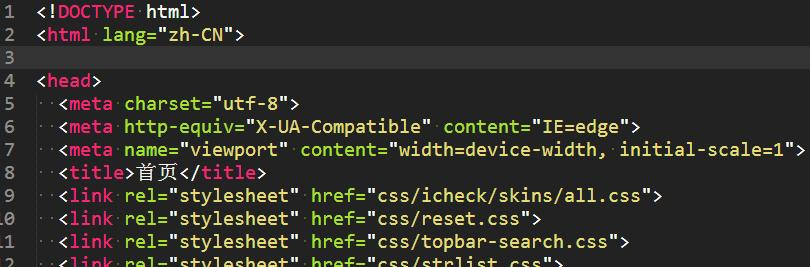
\includegraphics[width=10cm]{./img/index.jpg}
                  \caption{入口页示例}
                  \label{fig:index}
                \end{figure}

                其他的页面只需写入 html 片段即可, 如图 \ref{fig:tpl}

                \begin{figure}[H]
                  \centering
                  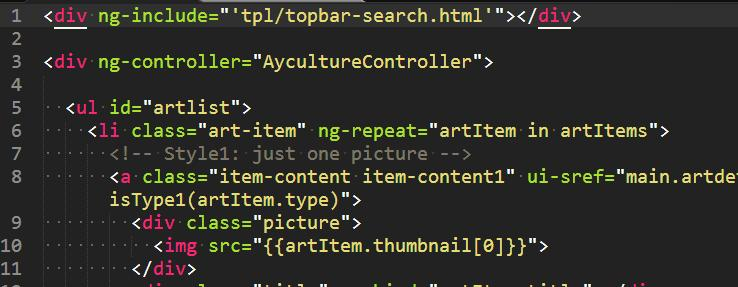
\includegraphics[width=10cm]{./img/tpl.jpg}
                  \caption{模板页示例}
                  \label{fig:tpl}
                \end{figure}

                路由的作用是:根据 url 控制加载相应的模板,通过 Angular 的 ui-router 模块实现,后面会具体讲解。如图 \ref{fig:router}

                \begin{figure}[H]
                  \centering
                  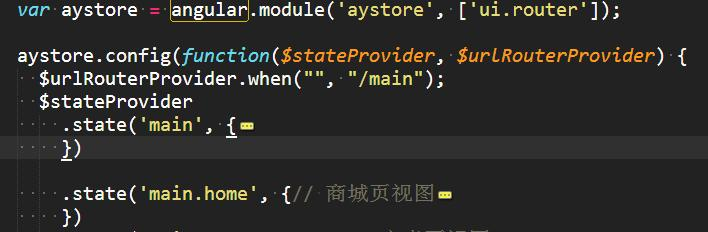
\includegraphics[width=10cm]{./img/router.jpg}
                  \caption{路由示例}
                  \label{fig:router}
                \end{figure}

            \subsubsection{控制器与模板引擎}
              \label{subsubsec:控制器与模板引擎}
                在没用 AngularJS 之前,如何向页面写入大量的数据对我来说是个非常棘手的问题,我之前是用的 jquery 实现的,利用了大量的 dom 操作和字符串拼接等,还利用了 h5 的 data-* 属性(防止引入过多的class或id),到最好实在难以维护,尤其是列表数据,如何让列表根据数据结构去展现是个比较麻烦的事情,如果用 jquery 实现的话,需要一个 for 循环,每个循环向模板中填充数据,填充数据的实现我也是靠 dom 操作,填充的数据包括标签的内容、标签的属性等,代码比较多,如图 \ref{fig:cmplx_jq_tpl},
                \begin{figure}[H]
                  \centering
                  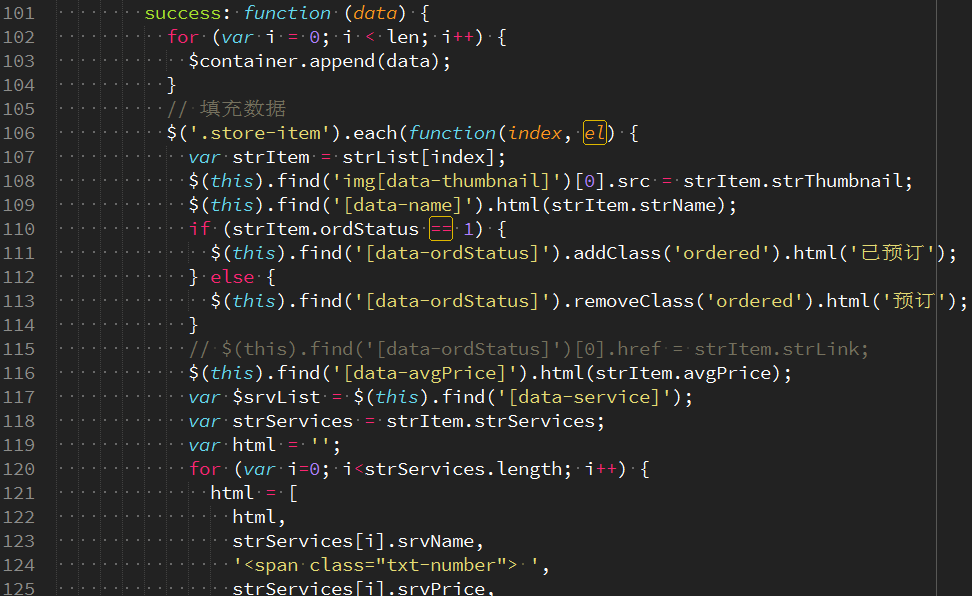
\includegraphics[width=12cm]{./img/cmplx_jq_tpl.png}
                  \caption{jQuery 填充模板的复杂性}
                  \label{fig:cmplx_jq_tpl}
                \end{figure}
                所以才选择去使用一款框架的。
                \par
                AngularJS 没有让我失望,AngularJS 利用控制器去向模板中填入数据,每个控制器都有自己的域———\$scope, 只需把数据挂载到 \$scope 上,然后在模板中直接引入用双大括号括起来的变量名即可,非常方便。
                如图:AngularJs 的模板引擎
                而且,对于列表的形式, AngularJS 有独特的循环模板指令——ng-repeat, 写法类似于 Js 的 for...in 循环,十分方便,简化了大量的代码。

            \subsubsection{依赖注入}
              \label{subsubsec:依赖注入}
                调用控制器时,传入的第二个参数是一个回调函数,这个回调函数中可以根据需要加载相应的服务,不需要按照顺序,AngularJS 会根据参数名自动确定参数,这样就只需一个函数,不需要管他的参数,是一种神奇的机制。

            \subsubsection{ui-router 模块}
              \label{subsubsec:ui_router_模块}
                本项目采用了 AngularJS 的一个 ui-router 插件来配置路由。ui-router 的一个路由由一下几部分组成:
                \begin{itemize}
                  \item 状态名
                  \item url
                  \item 模板文件(html 文件的路径或字符串)
                  \item 各个视图
                  \begin{itemize}
                    \item 某个视图
                    \item 视图的模板
                  \end{itemize}
                \end{itemize}
                \par
                ui-router 的核心在于:子路由与多重视图。一个路由对应一个模板,而一个模板文件里面又有多个视图: ui-view, 每个视图又可以插入模板。子路由写法为:father.child, 子路由直接继承父路由的模板文件,然后可以修改父路由的部分视图,这就为模板的模块化提供了一种解决方案, ui-router 由图 \ref{fig:ui_view} 所示。
                \begin{figure}[H]
                  \centering
                  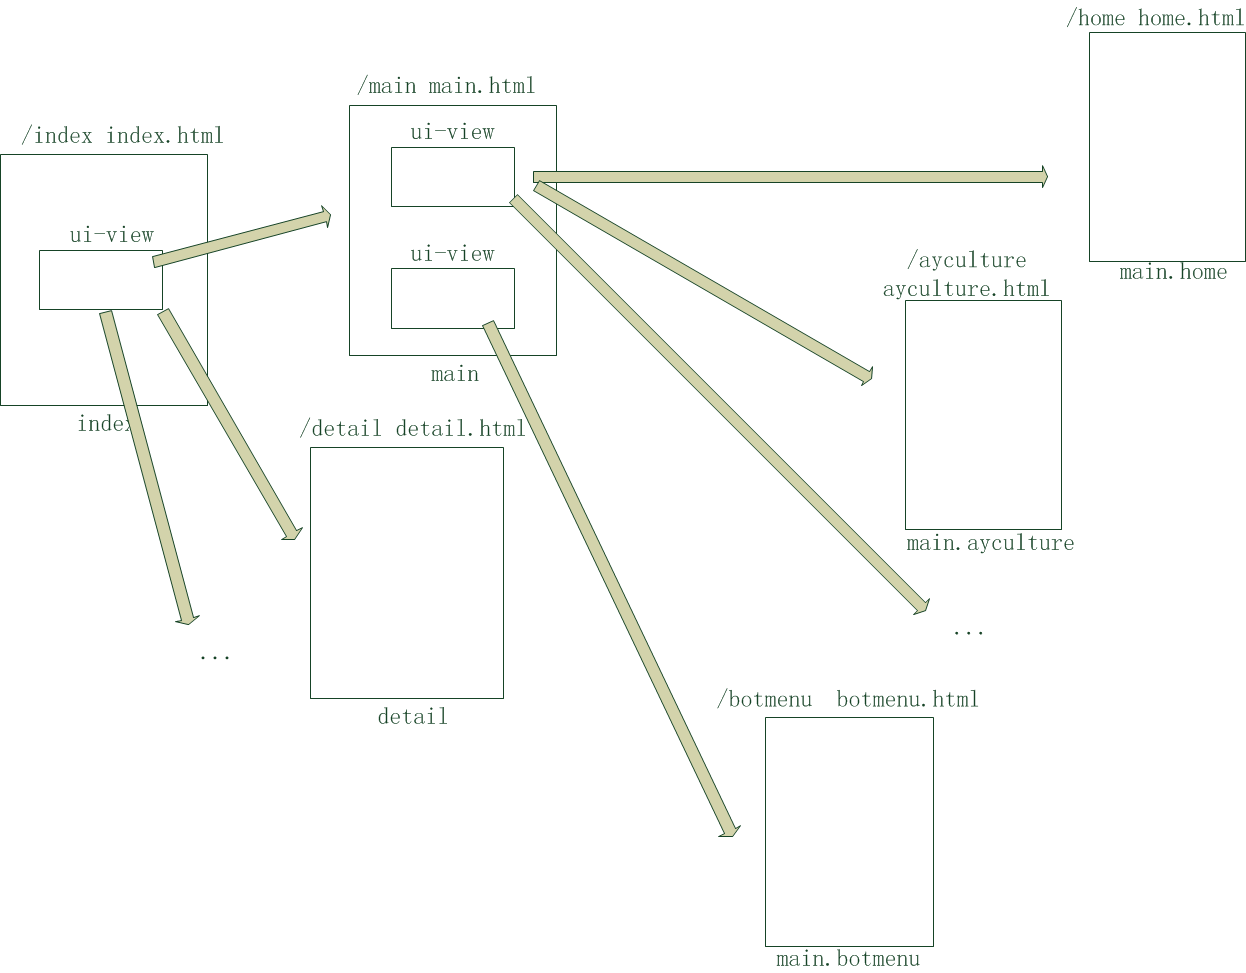
\includegraphics[width=\textwidth]{./img/ui_view.png}
                  \caption{ui-router 的示意图}
                  \label{fig:ui_view}
                \end{figure}
                项目的 9 个设计图中,有的页面有底部菜单,有的没有,因此就可以把有底部菜单的页面全都放在一个主路由下,项目路由的名称叫 main, 这些页面的路由只改变父路由的内容视图。其他的页面就每个单独配置路由即可。我把有底部菜单的页面全都配置成一个叫 "main" 路由的子路由,当URL跳转到这些页面时,这些页面的菜单部分不需要改动,只改动内容这个视图即可。

            \subsubsection{服务}
              \label{subsubsec:服务}
                AngularJS 的控制器有个特性,只会在需要的时候被实例化,而不需要时就会被销毁,每次切换路由或重新加载视图时,当前的控制器都会被 AngularJS 清除掉。而服务(Services)提供了一种在应用的整个生命周期保持数据的方法,能够在进程间通信。
                \par
                AngularJS 的服务分为两种,一种是内置服务,另一种是自定义服务。AngularJS 提供了一些内置服务,提供了一些常用的方法,例如
                \$timeout, \$http, \$factory等,我的项目中采用了 \$timeout 用于延时,这是为了解决 JS 异步加载的一个 bug,困扰了我好长时间;\$http 用于处理 http 请求,我的项目中需要向服务器请求商城列表、文章列表等,就会用到这个服务;\$factory 服务用来自定义服务,我的项目中自定了一个叫 DayAndTimeTest 的服务,用于根据艾灸服务的不同时段自动确定价格。

    \section{工具}
      \label{sec:工具}
        \subsection{Sublime Text 3}
          \label{subsec:sublime_text_3}
            Sublime Text 3 是一款非常强大的编辑器,如图 \ref{fig:sublime}, 目前是我最喜欢的编辑器,有诸多的优点。
            \par
            \textbf{漂亮}\, Sublime 本身的字体就很美观,目前我换成了 Source Code Pro 字体,这是目前我认为最漂亮的字体。
            \begin{figure}[H]
              \centering
              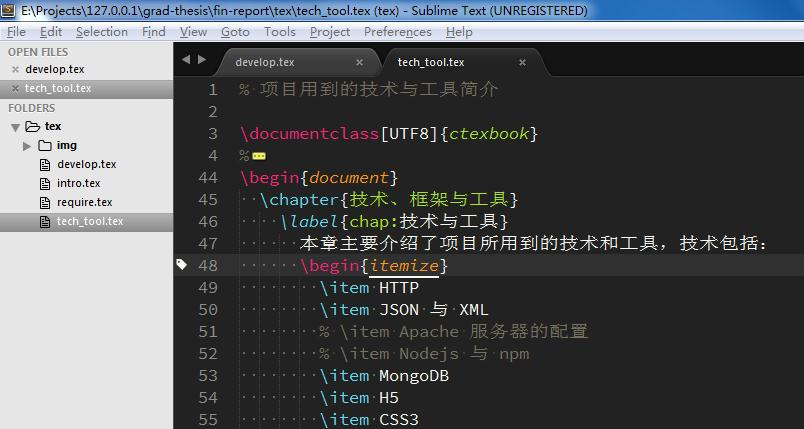
\includegraphics[width=10cm]{./img/sublime.jpg}
              \caption{Caption here}
              \label{fig:sublime}
            \end{figure}
            \textbf{轻量}\, Sublime Text 3 的安装包只有 8 MB,即使在我安装了大量的插件(40 多个)后也不到 150MB,相比于 IDE 更加轻量,因此速度也是飞快。一个 IDE 至少几百兆甚至一两G, 大量的功能用不上,Sublime 的功能是根据需要来安装相应的插件,因此是按需索取,有更强的定制性。
            \textbf{高效的操作}\, Sublime Text 官网中间就贴了一张动图,展示了 Sublime 的高效操作,如快速定位(文件、函数、某一行)、多光标编辑、快速选中单词和移动行等。

            \textbf{插件系统、代码片段}\, Sublime 有着众多的插件,基本上可以打造任何编程语言的环境,语法高亮、实时纠错、代码片段等,让写代码快得飞起。

        \subsection{Chrome}
          \label{subsec:chrome}
            Chrome 是 Google 公司出品的浏览器,如图 \ref{fig:chrome}
            \begin{figure}[H]
              \centering
              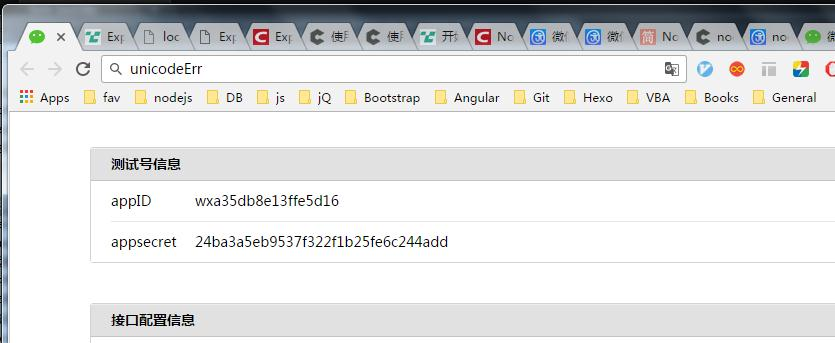
\includegraphics[width=10cm]{./img/chrome.jpg}
              \caption{Chrome 浏览器}
              \label{fig:chrome}
            \end{figure}
            功能强大,界面美观,兼容性好,有着强大的调试工具。Chrome 是前端开发必备的神器。浏览器的作用是渲染 HTML 和编译 JavaScript, HTML 在不断发展,不断增加新特性,这就要求浏览器的兼容性要好,同时 JavaScript 也在快速发展,浏览器此时作为编译引擎,性能要足够出色。
            \par
            Chrome 采用了 V8 引擎来编译 JavaScript ,是目前最快的编译引擎。同时,除了编译还要能够调试,Chrome 的调试功能也非常强大,如图 \ref{fig:chrome_debug}, 下面,我们就来详细谈谈 Chrome 的调试功能。
            \begin{figure}[H]
              \centering
              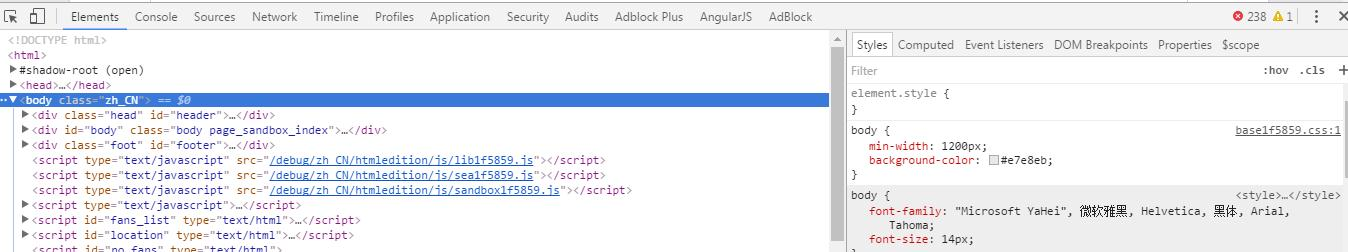
\includegraphics[width=\textwidth]{./img/chrome_debug.jpg}
              \caption{Chrome 的调试工具}
              \label{fig:chrome_debug}
            \end{figure}

            \subsubsection{Elements}
              \label{subsubsec:elements}
                我们看图 \ref{fig:chrome_debug} 中的几项菜单,第一个 Elements 是页面代码,可以方便的折叠和展开,坐上角的箭头一样的图标是用来审查(inspect)元素,如图 \ref{fig:cr_inspect},
                \begin{figure}[H]
                  \centering

                  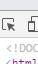
\includegraphics[width=2cm]{./img/cr_inspect.jpg}
                  \caption{Chrome 审查元素功能}
                  \label{fig:cr_inspect}
                \end{figure}
                翻译成捕捉更合适一点,因为它的功能是迅速定位元素在代码的位置,特别强大,如图 \ref{fig:cr_inspect1},
                \begin{figure}[H]
                  \centering
                  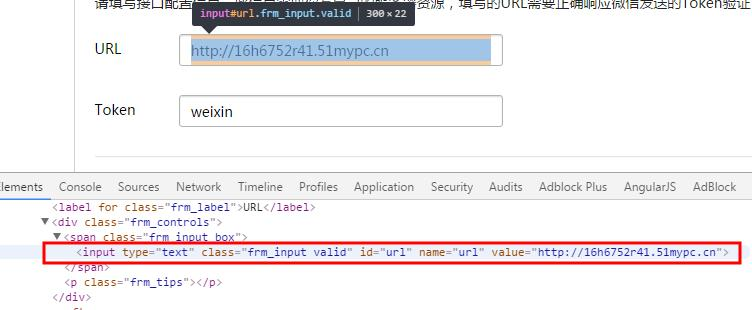
\includegraphics[width=12cm]{./img/cr_inspect1.jpg}
                  \caption{Chrome 定位元素的代码}
                  \label{fig:cr_inspect1}
                \end{figure}
                当点击审查元素的菜单后,我把鼠标移动到某个输入框上,Chrome 迅速为我定位到了其所在HTML代码处,同时右边还显示了对应的 CSS 样式,很强。
                \begin{figure}[H]
                  \centering
                  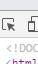
\includegraphics[width=2cm]{./img/cr_inspect.jpg}
                  \caption{Caption here}
                  \label{fig:figure1}
                \end{figure}

            \subsubsection{Console}
              \label{subsubsec:console}
                Console 即控制台,用于执行 javascript 语句和打印结果,如图 \ref{fig:cr_console},
                \begin{figure}[htbp]
                  \centering
                  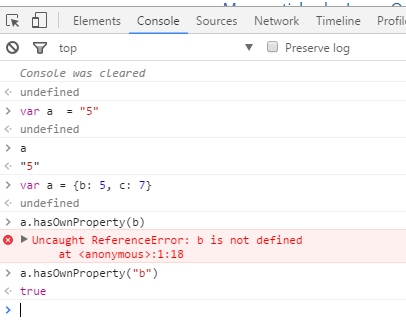
\includegraphics[width=8cm]{./img/cr_console.png}
                  \caption{控制台窗口}
                  \label{fig:cr_console}
                \end{figure}
                我一般用 Consolo 去测试一些 JavaScript 的方法、函数, dom 对象的一些方法以及测试 ajax 方法获取的数据是否正确。

            \subsubsection{Sources}
              \label{subsubsec:sources}
                Sources 是指加载的一些静态文件,如 html 文件,css 样式文件,图片,视频文件等,而加载的 js 文件可以进行断点调试,如图 \ref{fig:cr_sources}
                \begin{figure}[htbp]
                  \centering
                  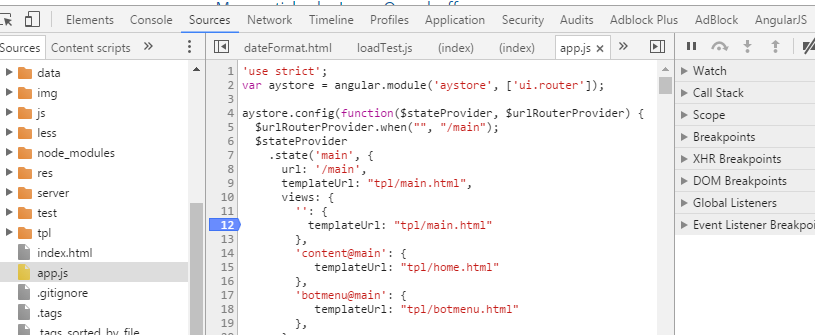
\includegraphics[width=12cm]{./img/cr_sources.png}
                  \caption{Sources}
                  \label{fig:cr_sources}
                \end{figure}
                变量的值还可以在当前执行的语句后显示出来。

            \subsubsection{Network}
              \label{subsubsec:network}
                Network 一栏主要是显示了资源的加载状况。打开调试工具后定位到 Network 一栏,此时刷新页面,就会看到下面出现一个列表,里面显示了各个资源的加载的时间、状态、类型、名字、方法等,如图 \ref{fig:cr_network}。
                \begin{figure}[htbp]
                  \centering
                  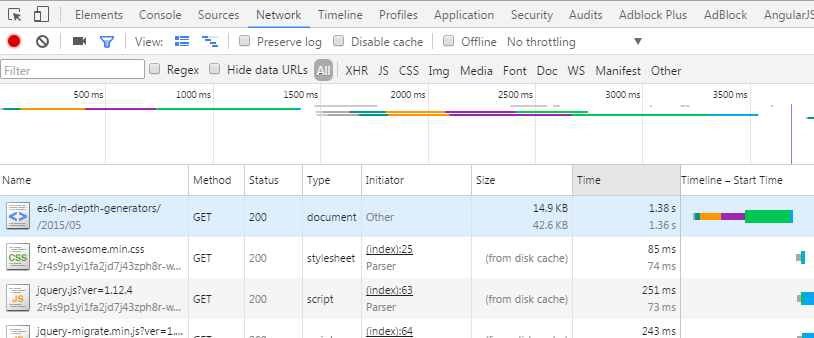
\includegraphics[width=12cm]{./img/cr_network.png}
                  \caption{Network}
                  \label{fig:cr_network}
                \end{figure}

            \subsubsection{Application}
              \label{subsubsec:application}
                Application 一栏主要与缓存有关,如图 \ref{fig:cr_application}
                \begin{figure}[H]
                  \centering
                  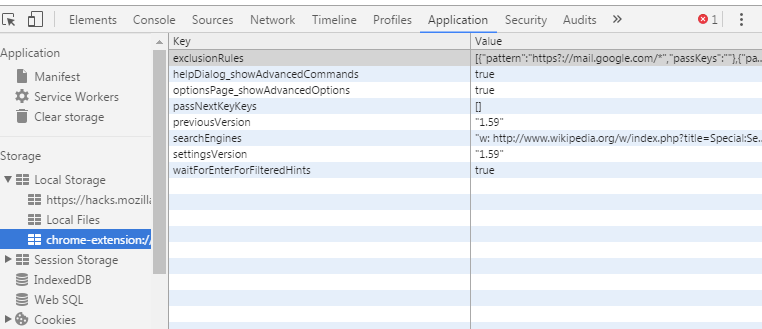
\includegraphics[width=12cm]{./img/cr_application.png}
                  \caption{application}
                  \label{fig:cr_application}
                \end{figure}
                左边 Application 目录下的 Manifest 保存了缓存文件的列表,Storage 目录下主要是本地存储技术,例如:
                \begin{itemize}
                  \item Local Storage
                  \item Session Storage
                  \item IndexedDB
                  \item WebSQL
                  \item Cookies
                \end{itemize}
                \par
                除了 Cookies,其他的存储方式都是 H5 新增的存储标准,容量一般都很大,例如 Local Storage 的容量可以达到 5MB, 而 Cookies 只有 4K,很多的网站开始尝试用 Local Storage 作为本地存储,而 IndexedDB 和 WebSQL 技术属于比较新的技术,还没有大面积使用。
                \par
                大量使用本地存储,对于服务器来说可以减轻负担,而对于客户端来说,减少了流量使用,提高了响应速度,Local Storage 我用来进行跨页数据传输问题,这只是方案之一,local Storage 的使用很方便,主要是 localStorage 对象,设置值用 localStorege.set('key', 'value') 或者 localStorege.key = value, 获取值用 localStorege.get('key') 或者 localStorege.key,因为 localStorage 也是一个对象,因此可以通过点或者中括号的方法获取或设置相应的值。
                \par
                以上介绍的功能是我在项目开发时常用的,调试非常方便,特别是在样式调试时的定位元素、实时修改属性值的时候,非常方便,而 JS 调试功能,如果是自己写的底层代码,即不用框架的话,调试起来是很方便的,会定位到相应的行,但是如果使用框架,问题就出来了,经常定位不到自己的代码中,而是定位到框架的代码中,如 angularjs 第 10500 行,此时就很头痛,只能把错误信息拿到网页去查询,这样的调试耗去了我大部分时间,针对框架调试的问题,我还没有找到好的方法。
                \par
                总之,Chrome 的调试工具无比强大,用好它可以大大缩短开发进度。

        \subsection{微信 Web 开发者工具}
          \label{subsec:微信_web_开发者工具}
            微信 Web 开发者工具是用来做微信开发的,实际上移动端的开发也可以用,如图 \ref{fig:wxweb}
            \begin{figure}[H]
              \centering
              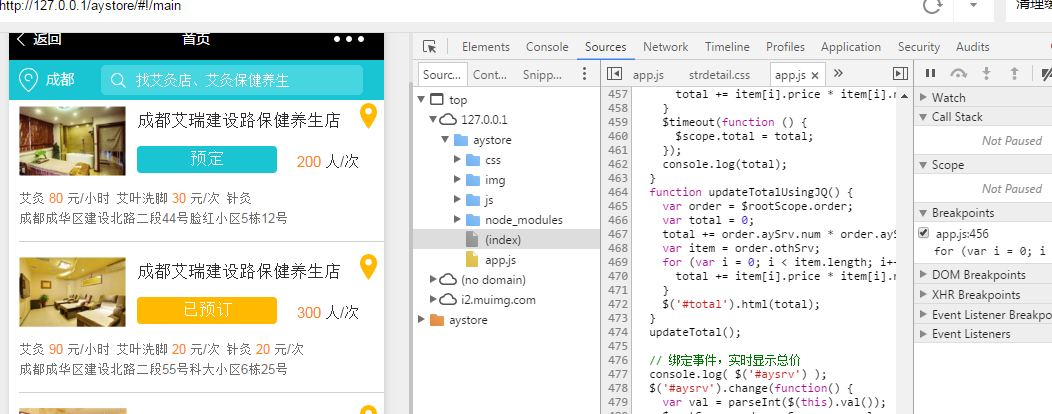
\includegraphics[width=12cm]{./img/wxweb.png}
              \caption{Caption here}
              \label{fig:wxweb}
            \end{figure}
            微信 Web 开发者工具采用的就是 Chrome 的调试工具,只不过只针对移动页面而已,不过也有其他的扩展,如 JSSDK 功能等。

        \subsection{Git}
          \label{subsec:git}
            Git 一款强大的版本控制工具,最早是用于 Linux 开发,由 Linux 系统的开发者 linus Trovals 研发。版本控制系统的目标是控制项目的版本,它可以记录你的每一次提交,因此你可以很方便的回到历史的版本,而不用去创建大量的备份,可以创建分支,团队协作开发等。Git 相对于其他的版本控制系统,更强大的地方在于本地仓库,每台设备都有一模一样的本地版本,不用担心中央服务器突然崩溃的问题。我个人用 Git 主要是用于版本同步,我有时在公司实习写的代码要和寝室的代码同步,简单的几行命令就可实现。

    \section{本章小结}
      \label{sec:技术与工具小结}
        本章主要介绍了我在项目开发中用到的技术和工具,以上只是列举了我自己用得到的工具,事实上,前端领域中还有大量的工具,包括很多效果库、框架、自动化工具构建、测试工具等。工欲善其事必先利其器,工具用得好可以大大提升开发速度,简化重复的劳动,我们应该积极去学习,尤其是在前端这个发展迅猛的行业。
